\documentclass[a4paper]{article}

\usepackage{polyglossia}
\setdefaultlanguage{russian}
\usepackage{fontspec}
\setmainfont{Times New Roman}
\newfontfamily\cyrillicfont{Times New Roman}
\newfontfamily\cyrillicfonttt{FreeMono}

\usepackage{graphicx}
\usepackage{float}
\usepackage{wrapfig}
\usepackage{tikz}
\usepackage{svg}

\usepackage{amsmath, amssymb}

\usepackage{hyperref}
\definecolor{urlcolor}{rgb}{0,0,1}
\definecolor{linkcolor}{rgb}{0,0,0.8}
\hypersetup{
  pdfborder=0 0 0,
  pdfstartview=FitH,
  linkcolor=linkcolor,
  urlcolor=urlcolor,
  colorlinks=true
}

\usepackage{caption}
\usepackage{geometry}
\geometry{left=2cm, right=2cm, top=2cm, bottom=2cm}

\usepackage{fancyhdr}
\usepackage{nicefrac}

\usepackage{xcolor}
\definecolor{strings}{rgb}{0,0.6,0}
\definecolor{comments}{rgb}{0,0.3,0}
\definecolor{numbers}{rgb}{0.5,0.5,0.5}
\definecolor{keywords}{rgb}{0.09,0.61,0.95}
\definecolor{background}{rgb}{0.97,0.97,0.97}

\usepackage{listings}

\lstdefinestyle{codestyle}{
    backgroundcolor=\color{background},
    commentstyle=\color{comments},
    keywordstyle=\color{keywords},
    stringstyle=\color{strings},
    numberstyle=\tiny\color{numbers},
    basicstyle=\ttfamily\footnotesize,
    breakatwhitespace=false,
    breaklines=true,
    captionpos=b,
    inputencoding=utf8,
    keepspaces=true,
    numbers=left,
    numbersep=5pt,
    showspaces=false,
    showstringspaces=false,
    showtabs=false,
    tabsize=2,
    extendedchars=true,
    literate=
      {а}{{\cyra}}1 {б}{{\cyrb}}1 {в}{{\cyrv}}1 {г}{{\cyrg}}1
      {д}{{\cyrd}}1 {е}{{\cyre}}1 {ж}{{\cyrzh}}1 {з}{{\cyrz}}1
      {и}{{\cyri}}1 {й}{{\cyrishrt}}1 {к}{{\cyrk}}1 {л}{{\cyrl}}1
      {м}{{\cyrm}}1 {н}{{\cyrn}}1 {о}{{\cyro}}1 {п}{{\cyrp}}1
      {р}{{\cyrr}}1 {с}{{\cyrs}}1 {т}{{\cyrt}}1 {у}{{\cyru}}1
      {ф}{{\cyrf}}1 {х}{{\cyrh}}1 {ц}{{\cyrc}}1 {ч}{{\cyrch}}1
      {ш}{{\cyrsh}}1 {щ}{{\cyrshch}}1 {ъ}{{\cyrhrdsn}}1 {ы}{{\cyrery}}1
      {ь}{{\cyrsftsn}}1 {э}{{\cyrerev}}1 {ю}{{\cyryu}}1 {я}{{\cyrya}}1
      {А}{{\CYRA}}1 {Б}{{\CYRB}}1 {В}{{\CYRV}}1 {Г}{{\CYRG}}1
      {Д}{{\CYR96}}1 {Е}{{\CYRE}}1 {Ж}{{\CYRZH}}1 {З}{{\CYRZ}}1
      {И}{{\CYRI}}1 {Й}{{\CYRISHRT}}1 {К}{{\CYRK}}1 {Л}{{\CYRL}}1
      {М}{{\CYRM}}1 {Н}{{\CYRN}}1 {О}{{\CYRO}}1 {П}{{\CYRP}}1
      {Р}{{\CYRR}}1 {С}{{\CYRS}}1 {Т}{{\CYRT}}1 {У}{{\CYRU}}1
      {Ф}{{\CYRF}}1 {Х}{{\CYRH}}1 {Ц}{{\CYRC}}1 {Ч}{{\CYRCH}}1
      {Ш}{{\CYRSH}}1 {Щ}{{\CYRSHCH}}1 {Ъ}{{\CYRHRDSN}}1 {Ы}{{\CYRERY}}1
      {Ь}{{\CYRSFTSN}}1 {Э}{{\CYREREV}}1 {Ю}{{\CYRYU}}1 {Я}{{\CYRYA}}1
}

\lstset{style=codestyle}

\begin{document}    

% Титульный лист
\begin{titlepage}
    \centering
    {\large Федеральное государственное автономное образовательное учреждение\par}
    {\large высшего образования\par}
    {\bfseries САНКТ-ПЕТЕРБУРГСКИЙ НАЦИОНАЛЬНЫЙ ИССЛЕДОВАТЕЛЬСКИЙ УНИВЕРСИТЕТ ИТМО\par}
    {\bfseries Факультет систем управления и робототехники\par}
    \vfill
    {\Large \bfseries Лабораторная работа №3\par}
    {\Large \bfseries Ускорение град. спуска, метод сопряженных градиентов \par}
    \vfill
    
    \begin{flushright}
        Студенты: Бахтаиров Р.А.,\\ Сайфуллин Д.Р. \\
        Группа:  R3243\\
        Преподаватель: Попов А.М.
    \end{flushright}
    \vfill
    Санкт-Петербург\\ 
    2025 г.
\end{titlepage}

\section{Введение}

В данной лабораторной работе исследуется ускорение базового метода градиентного спуска на примере трёх подходов:
\begin{enumerate}
    \item Метод тяжёлого шара (Heavy Ball), основанный на добавлении инерционного члена к классическому градиентному шагу.
    \item Метод Нестерова с постоянными коэффициентами, в котором используется заранее рассчитанный параметр ускорения на основе оценки числа обусловленности.
    \item Метод Нестерова с пересчитываемыми коэффициентами (FISTA-схема), обеспечивающий адаптивное изменение параметра ускорения на каждой итерации.
\end{enumerate}

Цель работы:
\begin{itemize}
    \item Реализовать и отладить перечисленные методы.
    \item Провести численные эксперименты на трёх классических задачах:
    \begin{enumerate}
        \item Квадратичные функции ($f(x)=\frac12 x^T A x - b^T x$).
        \item Почти квадратичная функция $f(x_1,x_2)=\frac12 x_1^2 + \frac14 x_2^4 - \frac12 x_2^2$.
        \item Функция Розенброка $f(x,y)=(1-x)^2 + 100(y-x^2)^2$.
    \end{enumerate}
    \item Эмпирически оценить области сходимости и скорость сходимости каждого метода.
    \item Сравнить численные результаты с аналитическими оценками и сделать выводы о практических преимуществах и ограничениях ускоренных методов.
\end{itemize}

\textit{Примечание: весь код для выполнения работы находится в файле \texttt{main.ipynb}.}

\section{Квадратичные функции}
Рассмотрим выпуклую квадратичную функцию
\[
f(x) \;=\; \tfrac12\,x^T A x \;-\; b^T x,
\]
где \(A \in \mathbb{R}^{n\times n}\) — симметричная положительно определённая матрица, \(b\in\mathbb{R}^n\).  

Ниже приведены графики сходимости четырёх методов на задаче минимизации при различных размерностях \(n\) и числах обусловленности \(\kappa(A)\).  
По оси \(x\) отложена итерация \(k\), по оси \(y\) — логарифм нормы ошибки \(\|x_k - x^*\|\).

\begin{figure}[H]
  \centering
  \begin{tabular}{cc}
    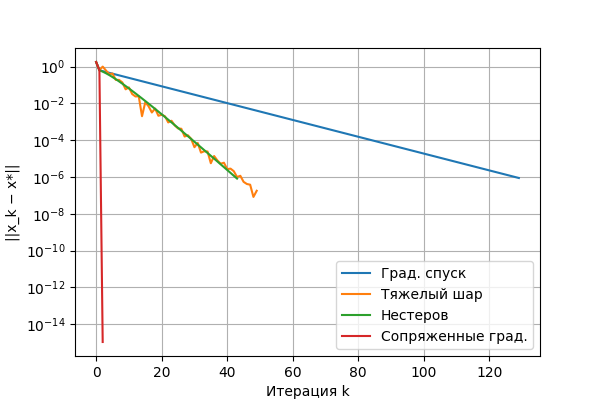
\includegraphics[width=0.45\textwidth]{images/task1_2_10.png} &
    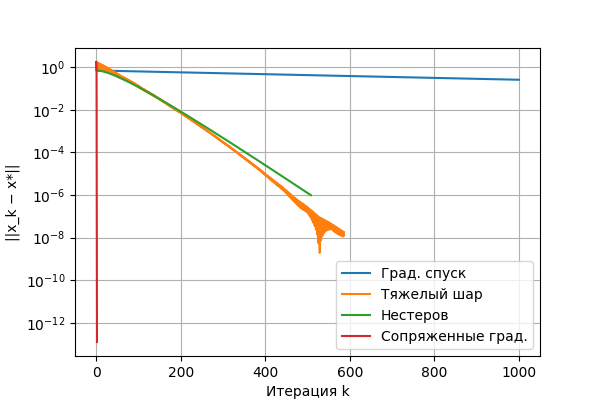
\includegraphics[width=0.45\textwidth]{images/task1_2_1000.png} \\[1ex]
    \(n=2,\ \kappa=10\) & \(n=2,\ \kappa=1000\) \\[2ex]
    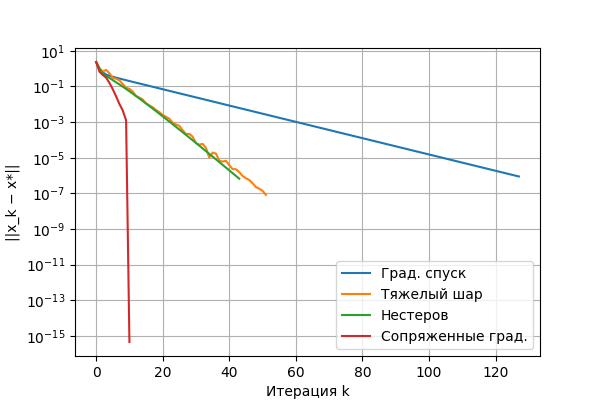
\includegraphics[width=0.45\textwidth]{images/task1_10_10.png} &
    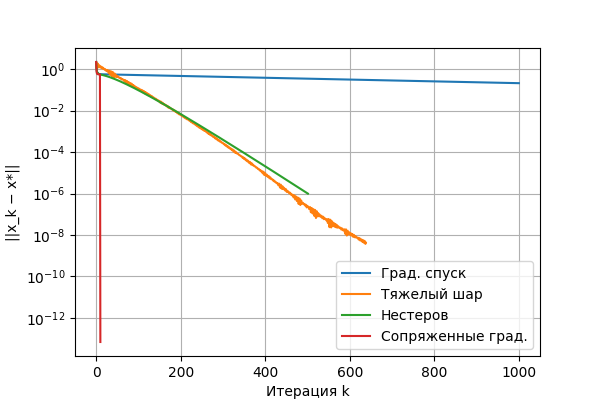
\includegraphics[width=0.45\textwidth]{images/task1_10_1000.png} \\[1ex]
    \(n=10,\ \kappa=10\) & \(n=10,\ \kappa=1000\) \\[2ex]
    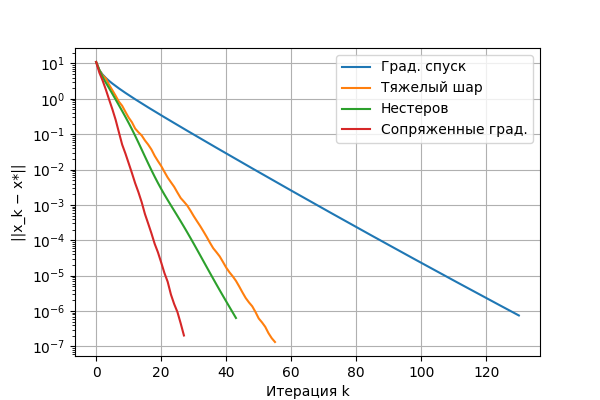
\includegraphics[width=0.45\textwidth]{images/task1_100_10.png} &
    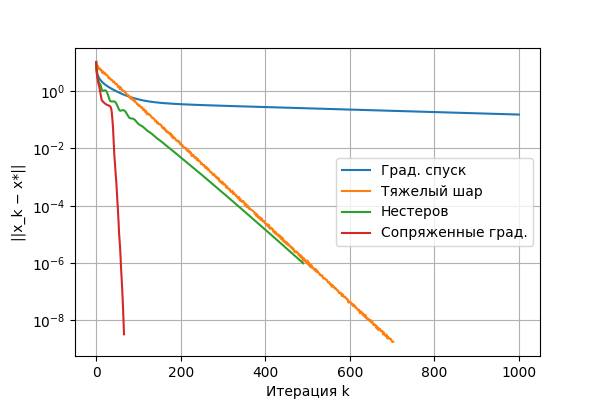
\includegraphics[width=0.45\textwidth]{images/task1_100_1000.png} \\[1ex]
    \(n=100,\ \kappa=10\) & \(n=100,\ \kappa=1000\) \\[2ex]
    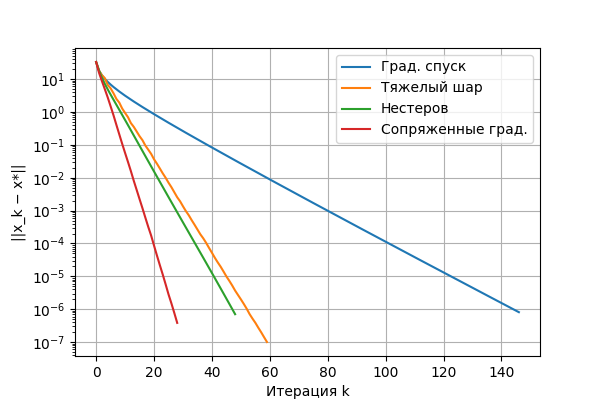
\includegraphics[width=0.45\textwidth]{images/task1_1000_10.png} &
    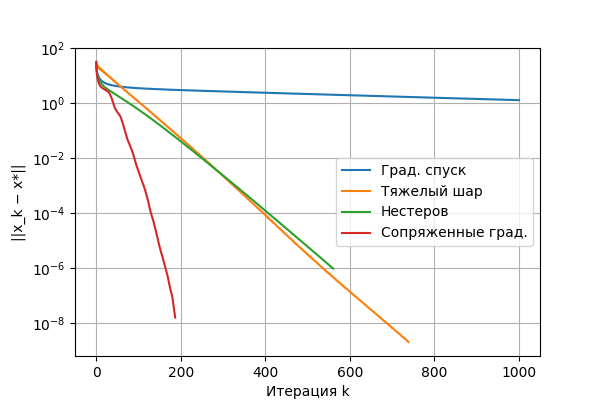
\includegraphics[width=0.45\textwidth]{images/task1_1000_1000.png} \\[1ex]
    \(n=1000,\ \kappa=10\) & \(n=1000,\ \kappa=1000\)
  \end{tabular}
  \caption{Сходимость методов: синий — градиентный спуск, оранжевый — Тяжелый шар, зелёный — Нестеров, красный — сопряжённые градиенты}
  \label{fig:quad_results}
\end{figure}

Проанализируем полученные графики:
\begin{itemize}
  \item \textbf{Градиентный спуск} (\(1/L\)-шаг) демонстрирует крайне медленную линейную сходимость, причём чем хуже обусловлена задача (\(\kappa\) больше), тем более пологая кривая.
  \item \textbf{Метод тяжёлого шара} и \textbf{Нестерова} дают существенное ускорение по сравнению с чистым Градиентным спуском:  
    \begin{itemize}
      \item При \(\kappa=10\) ускоренные методы сокращают число итераций почти вдвое.
      \item При \(\kappa=1000\) разрыв становится ещё более заметным: Градиентный спуск требует сотни шагов, а Тяжелый шар и Нестеров — всего десятки.
    \end{itemize}
    Их кривые часто накладываются, что свидетельствует о близкой эффективности при оптимальном подборе параметров.
  \item \textbf{Сопряжённые градиенты} сходятся за \(O(n)\) шагов практически независимо от \(\kappa\):  
    \begin{itemize}
      \item Для \(n=2\) метод достигает машинной точности уже за 2–3 итерации.
      \item При \(n=1000\) — за несколько сотен итераций.
    \end{itemize}
\end{itemize}

Исходя из наблюдений можем сделать следующие выводы:
\begin{enumerate}
  \item Для \emph{плохо обусловленных} квадратичных задач (\(\kappa\gg1\)) ускоренные методы (Тяжелый шар и Нестеров) значительно превосходят базовый Градиентный спуск, но при этом чувствительны к точности оценок \(L\) и \(\mu\).
  \item Метод сопряжённых градиентов оказывается наиболее \emph{универсальным} и \emph{оптимальным} в чисто квадратичном случае: сходимость за \(O(n)\) итераций вне зависимости от \(\kappa\).
  \item На практике при решении больших квадратичных систем предпочтительно сочетать анализ обусловленности (для выбора Тяжелого шара/Нестерова) или сразу применять Метод сопряженных градиентов, если доступен оператор умножения на \(A\).
\end{enumerate}

\section{Почти–квадратичная функция}

Рассмотрим функцию
\[
f(x_1, x_2) \;=\;\tfrac12 x_1^2 \;+\;\tfrac14 x_2^4 \;-\;\tfrac12 x_2^2.
\]

\begin{itemize}
  \item Стационарные точки находятся из условий
  \[
    \frac{\partial f}{\partial x_1}=x_1=0,
    \quad
    \frac{\partial f}{\partial x_2}=x_2^3 - x_2 = 0
    \;\Longrightarrow\;
    x_2\,(x_2^2-1)=0.
  \]
  \item Получаем три критические точки:
  \[
    (0,0)\quad\text{(седло)}, 
    \quad
    (0,1),\;(0,-1)\quad\text{(локальные минимумы)}.
  \]
  \item Гессиан
  \(\nabla^2 f=\begin{pmatrix}1&0\\0&3x_2^2-1\end{pmatrix}\)
  даёт знакоположительность в точках \((0,\pm1)\) и знакопеременность в \((0,0)\).
\end{itemize}

Построим графики функции и её уровней:
\begin{figure}[H]
  \centering
  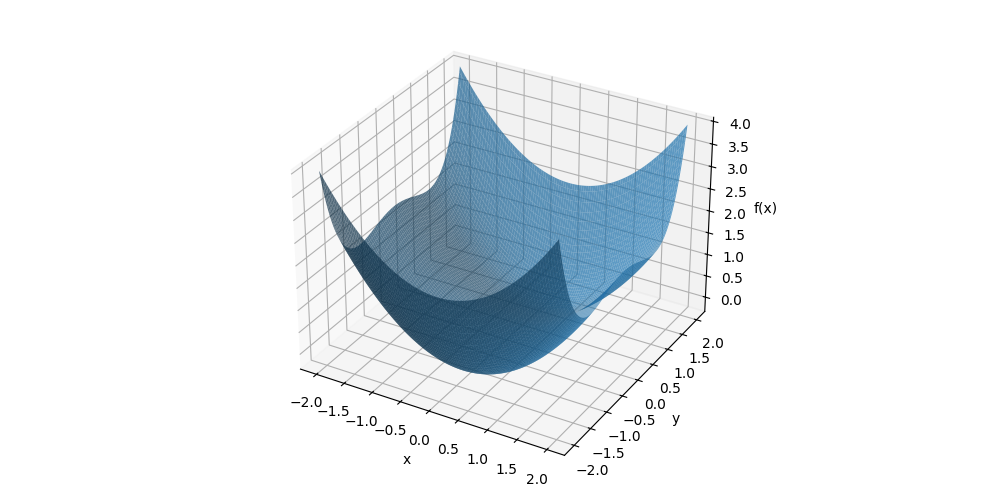
\includegraphics[width=\textwidth]{images/task2_surf.png}
  \caption{Поверхность функции \(f(x_1,x_2)\).}
\end{figure}

\begin{figure}[H]
  \centering
  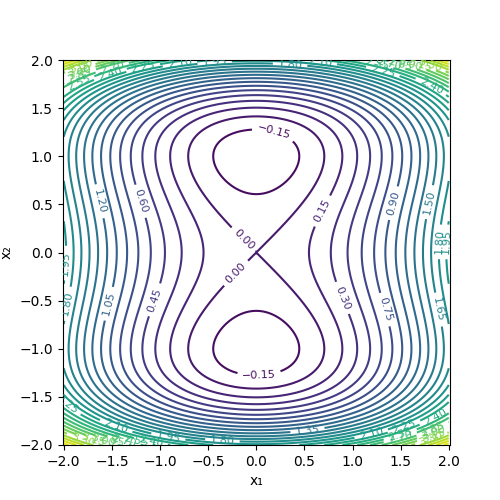
\includegraphics[width=0.6\textwidth]{images/task2_min.png}
  \caption{Контурный график функции.}
\end{figure}

Теперь проверим на сходимость три метода и построим графики. Запустим их из начальной точки \((1.5,1.5)\):
\begin{itemize}
  \item Метод тяжёлого шара,
  \item Метод Нестерова с постоянным \(\beta\),
  \item Метод Флетчера–Ривза.
\end{itemize}

\begin{figure}[H]
  \centering
  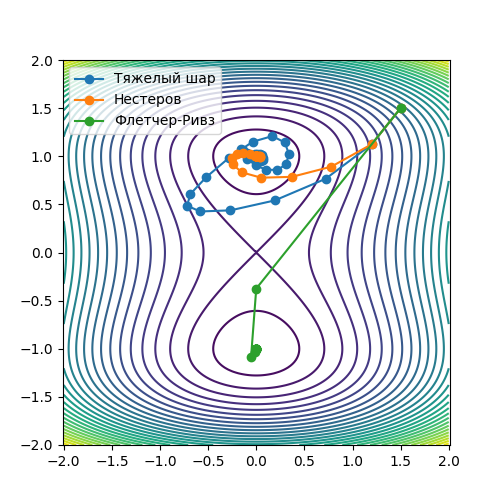
\includegraphics[width=0.6\textwidth]{images/task2_paths.png}
  \caption{Траектории трёх методов на контурном графике функции.}
  \label{fig:task2_paths}
\end{figure}

Анализируя график мы можем сделать следующие выводы:

\begin{enumerate}
  \item Все три метода успешно сходятся к ближайшему локальному минимуму \((0,\pm1)\), обходя седло в \((0,0)\).
  \item Метод Тяжелого шара демонстрирует умеренные колебания вокруг траектории, но быстро выходит на минимум.
  \item Нестеров с постоянным \(\beta\) идёт более плавно, чем Метод Тяжелого шара.
  \item Метод Флетчера–Ривза строит наиболее прямую траекторию, однако при слабой выпуклости функции может проходить ближе к седлу, что заметно на втором участке пути.
  \item По эмпирическим измерениям числа итераций до сходимости:
  \[
    \text{Метод тяжёлого шара}\approx 25,\quad
    \text{Метод Нестерова}\approx 20,\quad
    \text{Метод Флетчера–Ривза}\approx 5.
  \]
\end{enumerate}

\section{Функция Розенброка}

Рассмотрим классическую двухмерную задачу
\[
f(x,y) = (1 - x)^2 + 100\,(y - x^2)^2,
\]
которая известна своей узкой «долиной» и плохо обусловленным гессианом.

В этой части работы необходимо:
\begin{enumerate}
  \item Реализовать метод Нестерова в двух версиях:
    \begin{itemize}
      \item \emph{с постоянным} коэффициентом ускорения \(\beta\);
      \item \emph{с динамическим}.
    \end{itemize}
  \item Построить график сравнения двух версий Нестерова.
  \item Реализовать не менее трёх модификаций нелинейного метода сопряжённых градиентов:
    \(\beta^{\rm FR}, \beta^{\rm PR}, \beta^{\rm HS}\).
  \item Сравнить эти три CG-варианта и обычный градиентный спуск.
\end{enumerate}

\paragraph{Нестеров: постоянный vs динамический}  
На графике ниже показаны кривые при итерациях для двух версий:
\begin{itemize}
  \item \emph{const} (синий);
  \item \emph{dynamic} (оранжевый).
\end{itemize}

\begin{figure}[H]
  \centering
  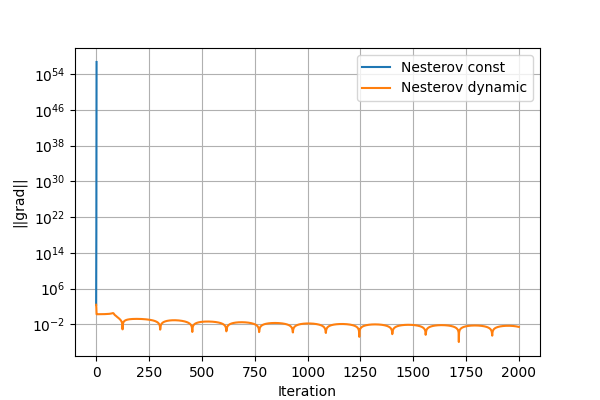
\includegraphics[width=0.6\textwidth]{images/task3_nesterov_comp.png}
  \caption{Сходимость метода Нестерова на функции Розенброка}
\end{figure}

\begin{enumerate}
  \item При старте (\(k<10\)) обе версии сходятся аналогично быстро, однако константная схема затем почти выравнивается и перестаёт снижаться, что видно по «выпрямлению» синей кривой.
  \item Динамическая версия демонстрирует регулярные «провалы» — резкие локальные уменьшения нормы градиента в моменты обновления \(\beta_k\), после чего метод вновь стабилизируется на новом уровне.
  \item В долгосрочной перспективе (\(k>200\)) только динамический Нестеров продолжает плавное снижение, тогда как версия const зашла в застой и не может преодолеть Розенброка.
\end{enumerate}

\paragraph{Модификации Метода сопряженных градиентов и Метод сопряженных градиентов}  
На графике ниже сравниваются:
\[
\text{Метод градиентного спуска},\quad
\text{Метод Флетчера–Ривза},\quad
\text{Метод Полак-Рибье},\quad
\text{Метод Хестинс-Штифель},
\]

\begin{figure}[H]
  \centering
  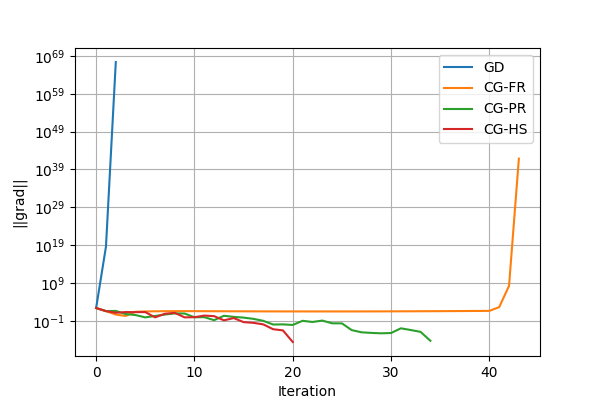
\includegraphics[width=0.6\textwidth]{images/task3_cg_variants.png}
  \caption{Сравнение Градиентного спуска и трёх модификаций Метода сопряженных градиентов на Розенброке}
\end{figure}

\begin{enumerate}
  \item \textbf{GD} (синяя кривая) резко замедляется после нескольких шагов и вблизи минимума снижает скорость убывания градиента в несколько порядков.
  \item \textbf{CG-FR} (оранжевая) сначала сходится быстро, но затем «взрывается» (возникает резкий рост), что указывает на неустойчивость метода FR без жёсткого контроля шага.
  \item \textbf{CG-PR} (зелёная) показывает стабильное и монотонное уменьшение до малых значений, без значительных всплесков.
  \item \textbf{CG-HS} (красная) сходится чуть быстрее PR и тоже сохраняет плавность траектории.
\end{enumerate}

При попытке применить стандартный линейный поиск в SciPy мы столкнулись с несколькими трудностями:
\begin{itemize}
  \item overflow в вычислении градиента: при агрессивном шаге \(x\) «улетал» в области, где \(y - x^2\) большим образом увеличивался.
  \item LineSearchWarning: алгоритм не всегда сходился, выдавая предупреждения.
  \item После нескольких десятков итераций возникали NaN и inf из-за потери численной устойчивости.
\end{itemize}

Теперь сделаем выводы по всем экспериментам на функции Розенброка:

\begin{itemize}
  \item Версия Нестерова с динамическим \(\beta\) оказалась более устойчивой и обеспечила стабильную сходимость, несмотря на резкие «впадины» градиента.
  \item Из трёх CG-модификаций \(\beta^{\rm PR}\) и \(\beta^{\rm HS}\) работают заметно лучше, чем \(\beta^{\rm FR}\), демонстрируя быструю и плавную сходимость до \(<10^{-6}\).
  \item Градиентный спуск без ускорения слишком медленный и быстро теряет точность из-за плохого баланса кривизны вдоль Розенброка.
  \item Для Розенброка предпочтительнее сочетать динамический Нестеров или PR/HS-версию CG с аккуратным линейным поиском; FR и фиксированный Нестеров могут потребовать значительной ручной настройки параметров.
\end{itemize}

\section{Общий вывод}
В ходе работы мы пришли к следующим выводам:
\begin{enumerate}
  \item \textbf{Ускоренные методы vs классический градиентный спуск.}
    \begin{itemize}
      \item Метод тяжелого шара и метод Нестерова демонстрируют значительное ускорение по сравнению с градиентным спуском на плохо обусловленных функциях.
      \item Для квадратичных задач с большим числом обусловленности (\(\kappa\gg1\)) оба метода сокращают число итераций в несколько раз, но требуют точных оценок \(L\) и \(\mu\).
      \item На «почти–квадратичной» и Розенброке Нестеров с динамическим параметром (\(\beta_k\)) показывает большую устойчивость и возможность выхода из плато по сравнению с фиксированной версией.
    \end{itemize}

  \item \textbf{Методы сопряжённых градиентов.}
    \begin{itemize}
      \item В строгом квадратичном случае CG-метод сходится за \(O(n)\) итераций, практически независимо от \(\kappa(A)\), что делает его оптимальным выбором при доступности операций с \(A\).
      \item Среди нелинейных CG-модификаций для функции Розенброка версии PR и HS выигрывают у FR благодаря большей численной устойчивости и отсутствию «взрывов» градиента.
    \end{itemize}

  \item \textbf{Численные тонкости и практические рекомендации.}
    \begin{itemize}
      \item Линейный поиск по Армихо–Вольфу может не сходиться на сильно негладких площадках (особенно для FR), поэтому для надёжности стоит применять backtracking или ограничивать шаг вручную.
      \item На функциях с узкими «долинами» (Розенброк, почти–квадратичная) полезна визуализация траекторий и анализ плато, чтобы скорректировать параметры \(\alpha\) и \(\beta\).
      \item В реальных приложениях сочетание адаптивных ускорений с аккуратным линейным поиском даёт наилучшее соотношение скорости сходимости и устойчивости.
    \end{itemize}
\end{enumerate}
\end{document}
